%%=============================================================================
%% Conclusie
%%=============================================================================

\chapter{Conclusie}%
\label{ch:conclusie}

% TODO: Trek een duidelijke conclusie, in de vorm van een antwoord op de
% onderzoeksvra(a)g(en). Wat was jouw bijdrage aan het onderzoeksdomein en
% hoe biedt dit meerwaarde aan het vakgebied/doelgroep? 
% Reflecteer kritisch over het resultaat. In Engelse teksten wordt deze sectie
% ``Discussion'' genoemd. Had je deze uitkomst verwacht? Zijn er zaken die nog
% niet duidelijk zijn?
% Heeft het onderzoek geleid tot nieuwe vragen die uitnodigen tot verder 
%onderzoek?

% Wat zijn de requirements die in de POC zijn voldaan en welke dienen nog verricht te worden? 

% Conclusie, huidige stand, toekomst visie?

Deze bachelorproef richtte zich op het ontwikkelen van een proof of concept voor een BibLaTeX-compatibele linter, gebaseerd op de bestaande \texttt{bibl}-tool, een linter voor BibTeX. Door de keuze voor Python als programmeertaal en de solide structuur van \texttt{bibl}, is een functionele en effectieve linter gerealiseerd die BibLaTeX-bestanden kan analyseren en valideren.

Tijdens de ontwikkeling en testen van deze linter is gebleken dat de tool over het algemeen betrouwbaar en consistent is, en nauwkeurige resultaten levert. Dankzij feedback van de promotor, medestudenten zijn diverse bugfixes doorgevoerd, wat heeft bijgedragen aan de verbetering van de tool zodat er onder andere minder foutieve detecties voorkomen. Hoewel er nog enkele mankementen zijn, worden deze actief gemeld via GitHub 'issues' en voortdurend aangepakt. Dit iteratieve proces zorgt ervoor dat de linter steeds verder wordt verbeterd en dat er ruimte blijft voor het toevoegen van extra functionaliteiten in de toekomst. Dit toont de doeltreffendheid van de linter en de waarde van een iteratief ontwikkelingsproces.

Er kan geconcludeerd worden dat het resultaat van dit project  positief is: de linter functioneert naar behoren en kan effectief worden ingezet als analysetool voor BibLaTeX-bestanden; zeker binnen de HOGENT-omgeving, gezien de regels de voorkeuren van HOGENT\footnote{\url{www.hogent.be}} respecteert. Deze tool stelt gebruikers in staat om consistentie en validiteit in hun bronvermeldingen te waarborgen, wat essentieel is voor academische werken. Dankzij de bekendmaking van de tool door de promotor en docent te HOGENT aan medestudenten, kon de tool al getest worden. Eén van deze medestudenten heeft een schermafbeelding voorzien waaruit de effectiviteit van \texttt{bibla} aangetoond kan worden, zie \ref{fig:bibla-is-useful}.
\\
\\
Samenvattend biedt \texttt{bibla} een meer uitgebreide en gedetailleerde set regels die beter zijn afgestemd op de eisen van BibLaTeX in vergelijking met \texttt{bibl}. De aanvullende en aangepaste regels zorgen voor een grotere nauwkeurigheid en consistentie in de verwerking van bibliografische vermeldingen. Door het volgen van deze regels kunnen gebruikers ervoor zorgen dat hun BibLaTeX-bestanden voldoen aan de huidige standaarden en best practices; die voor deze usecase werden opgelegd door HOGENT.

\begin{figure}[ht]
    \centering
    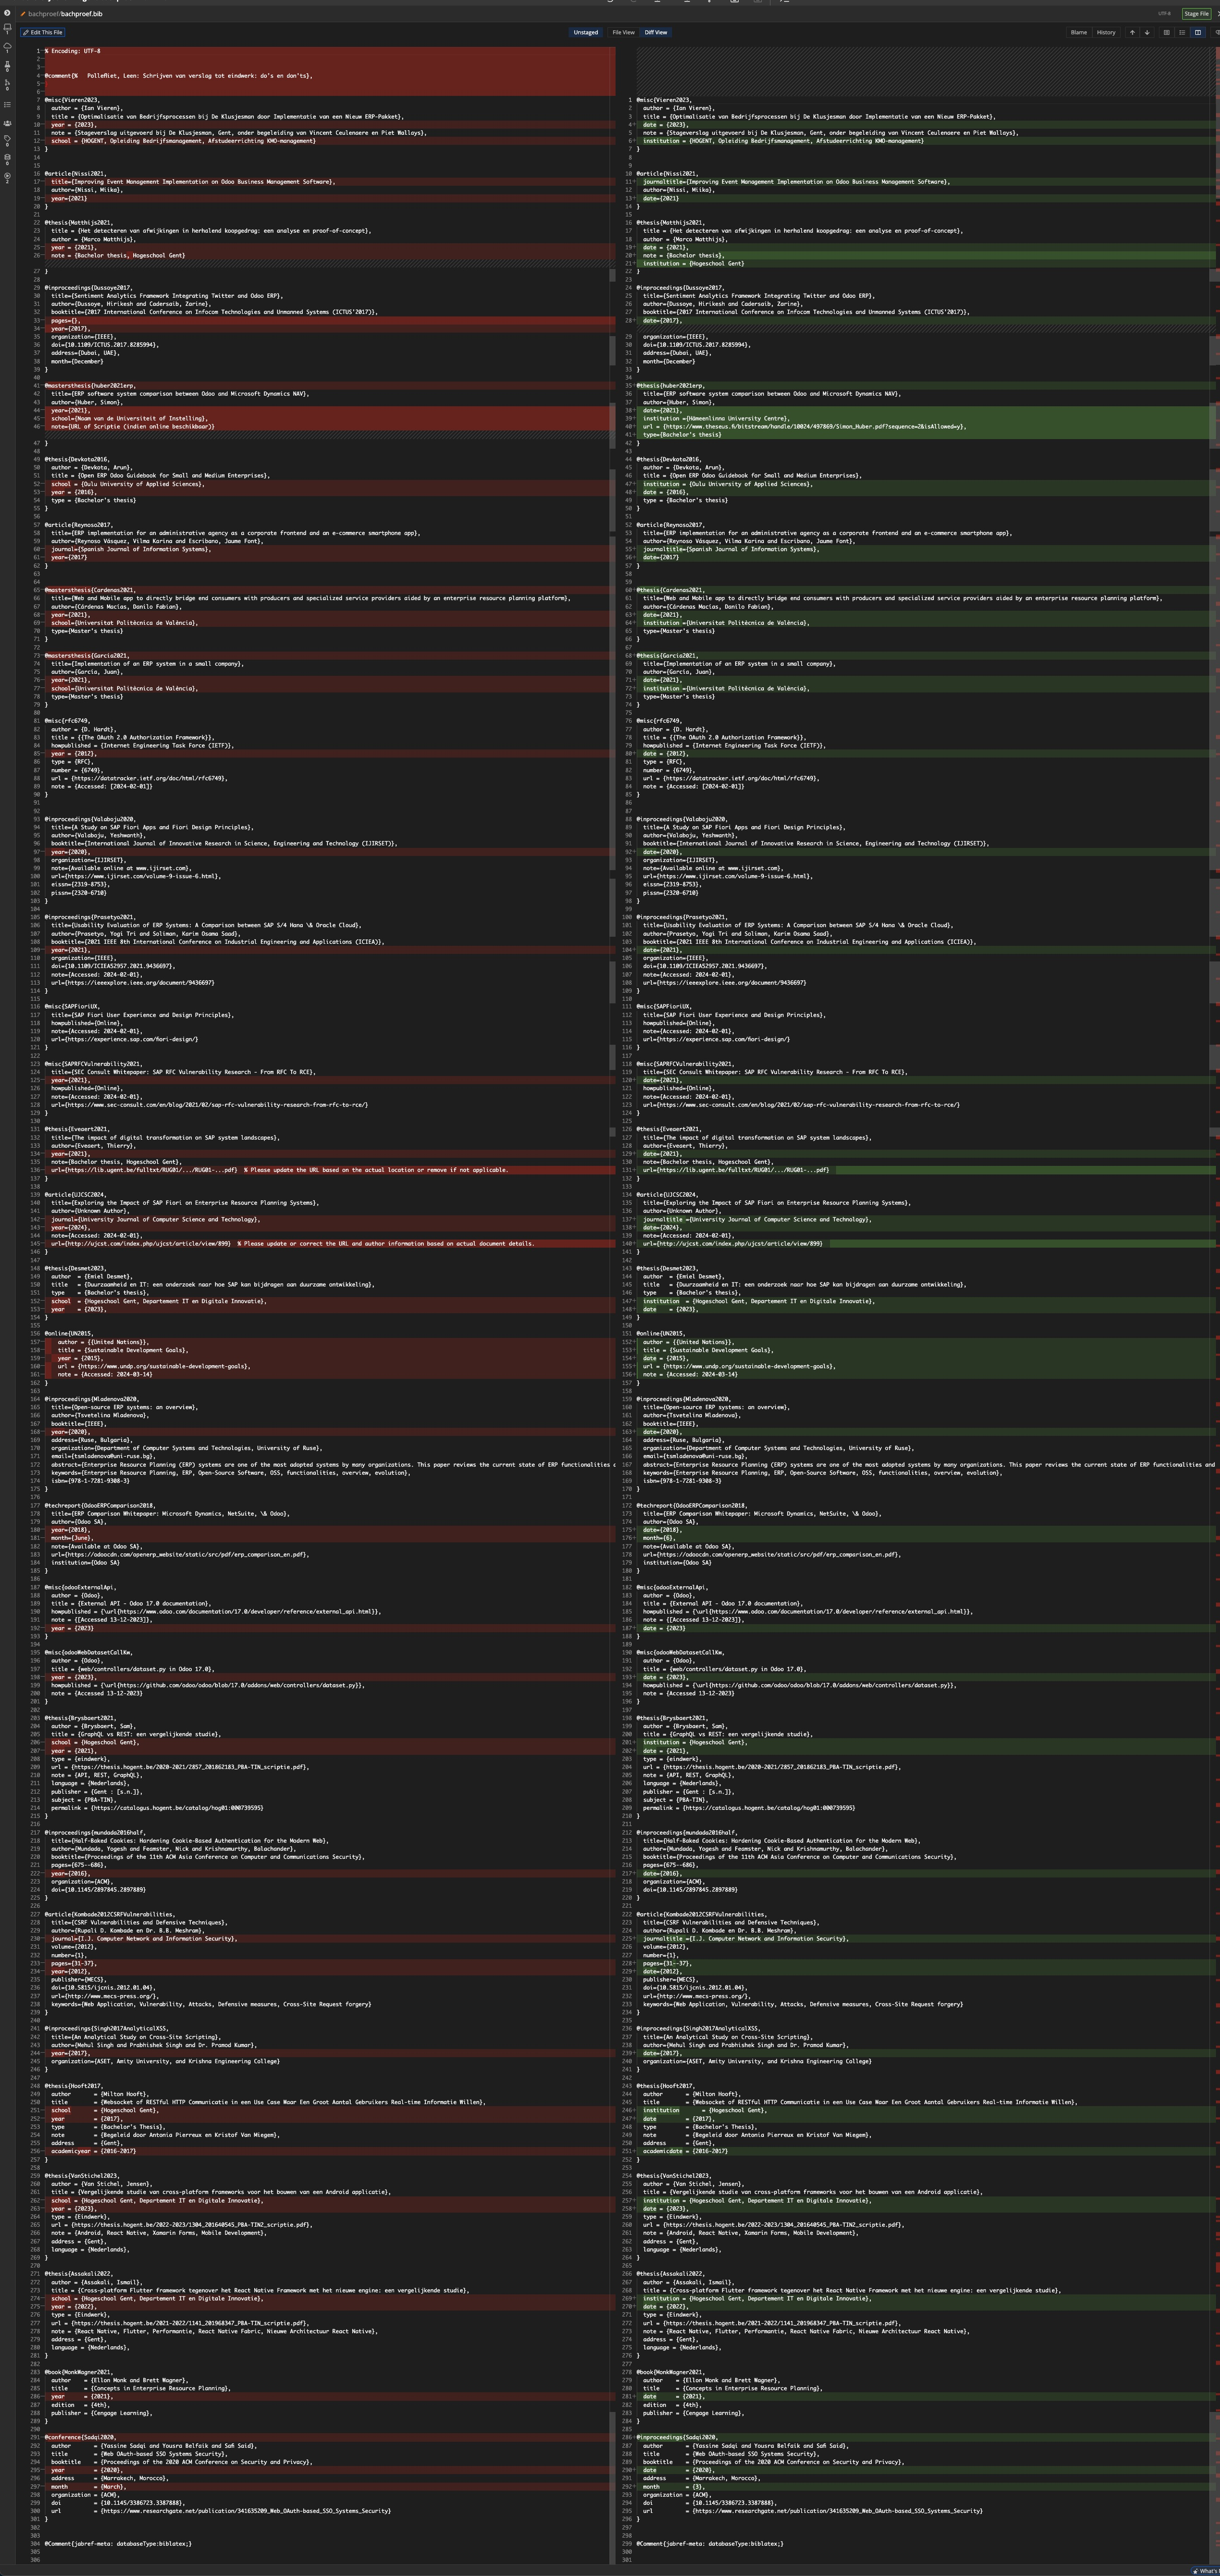
\includegraphics[width=0.7\textwidth]{./files/bibla_is_useful.jpeg}
    \caption[Effectiviteit bibla]{Deze afbeelding toont de \textbf{capaciteiten} van \textbf{bibla}. Een gebruiker heeft dit gedeeld, op de afbeelding kan het rode gezien worden als wat weggehaald werd en het groene als wat er in de plaats bijgekomen of ter vervanging is. Hoewel de afbeelding wat enigzins onduidelijk is, kunnen de aantal veranderingen die diende te gebeuren wel waargenomen worden. Dit illustreert het \textbf{aantal fouten} waarvan docenten - \textbf{per student} - bespaart zullen worden om ze iedere keer zelf aan te moeten halen en anderzijds heeft deze gebruiker nu een correctere bibliografie.}
    \label{fig:bibla-is-useful}
\end{figure}

\subsection{Toekomstvisie}
Het gebruik van \texttt{bibla} als de standaard bronvermeldingsanalysetool binnen HOGENT is een veelbelovende stap. Door de implementatie van \texttt{bibla} zullen studenten en docenten profiteren van een uniforme en betrouwbare methode om BibLaTeX-bestanden te controleren. Dit zal de kwaliteit van academische werken verbeteren en de werkdruk verlagen doordat veelvoorkomende fouten automatisch worden gedetecteerd.

De ontwikkeling van \texttt{bibla} staat echter niet stil. Nieuwe features en regels zullen blijven worden toegevoegd om de functionaliteit van de linter uit te breiden. Dit omvat bijvoorbeeld het toevoegen van extra types bronvermeldingen en het verbeteren van bestaande regels om nog nauwkeuriger te zijn. Daarnaast zullen eventuele nieuwe bugs worden aangepakt en opgelost om ervoor te zorgen dat de linter zo feilloos mogelijk kan werken.

Met \texttt{bibl} als stevige fundering was het mogelijk om \texttt{bibla} te ontwikkelen. De modulaire en uitbreidbare architectuur van \texttt{bibl} heeft bijgedragen aan een soepel ontwikkelproces en biedt een solide basis voor verdere uitbreidingen. Deze fundering zorgt ervoor dat \texttt{bibla} niet alleen nu, maar ook in de toekomst een waardevol hulpmiddel zal blijven voor de academische gemeenschap van HOGENT.

\subsection{Aanbevelingen}

Voor toekomstige ontwikkelaars en gebruikers van \texttt{bibla} zijn de volgende aanbevelingen relevant:
\begin{itemize}
  \item \textbf{Documentatie}: Zorg voor uitgebreide documentatie voor gebruikers om hen te helpen het meeste uit de tool te halen.
  \item \textbf{Feedback Verzamelen}: Blijf feedback verzamelen van gebruikers om de tool verder te verbeteren en aan te passen aan hun behoeften.
  \item \textbf{Community Betrokkenheid}: Moedig betrokkenheid van de academische gemeenschap aan om bij te dragen aan de ontwikkeling van nieuwe regels en eventuele features.
\end{itemize}

Met deze punten zal \texttt{bibla} zich kunnen blijven ontwikkelen en bijdragen aan de verbetering van academische publicaties zowel binnen, als buiten HOGENT.
